%-----------------------------------------------------------------
%	POWER DISSIPATION INDEX (PDI)
%	!TEX root = ./../main.tex
%-----------------------------------------------------------------
\subsection{PDI analysis}\label{sec:pdi-stats}

\subsubsection{PDI calculation}\label{ssec:pdi-calc}
After reading and cleaning the raw HURDAT2 data sets, calculating the $PDI$ using \eqref{eq:pdi-bis} is a straightforward process. To accomplish this, we created a function that transforms an observation data frame (\inline{hurr.obs}) into a new $PDI$ data frame (\inline{hurr.obs.pdi}) by grouping all the observation records by storm ID and summarising the product $v_{t}^{3} \Delta t$, and the maximum sustained wind speed during the storm's lifetime (this will allow us to filter tropical-cyclones by category). An important thing to take into account here is that, since the wind speed data is expressed in knots, we need to manually convert them into the International System of Units ($\SI{1}{\knot} = \SI{0.514}{\m\per\s}$):
\begin{lstlisting}[caption=Function to calculate a $PDI$ data frame, label=snp:hurdat-pdis]
get_pdis <- function(hurr.obs){
	hurr.obs.pdi <- hurr.obs %>%
		group_by(storm.id, storm.name, n.obs) %>%
		summarise(storm.pdi = sum(conv_unit(wind, "knot", "m_per_sec")^3 * conv_unit(6, "hr", "sec")),
							max.wind = max(wind)) %>%
		mutate(storm.duration = n.obs * conv_unit(6, "hr", "sec")) %>%
		mutate(storm.year = substring(storm.id, 5, 9)) %>%
		filter(storm.pdi != "NA") %>%
		filter(storm.pdi != 0)
	hurr.obs.pdi <- hurr.obs.pdi[c("storm.id", "storm.name", "n.obs", "storm.duration", "storm.pdi", "max.wind", "storm.year")]
	return(hurr.obs.pdi)
}
\end{lstlisting}

An important aspect to consider about the hurricane season of the tropical-cyclones is that they do not always start and end in the same year (e.g., the hurricane season for the Southwest Pacific Ocean is December--April \cite{Webster2005}). Although this is not our case (as depicted in table~\ref{tab:act-windows}), for the sake of reproducibility and completeness, we read the storm year directly from the storm ID instead of the \inline{date.time}; doing this would result in having two entries for such cases if we did \inline{group_by(storm.id, storm.name, n.obs, date.time)}.

%-----------------------------------------------------------------
\subsubsection{Resulting data structure}
In table~\ref{hd:pdi-head} we show the structure of the \inline{hurr.natl.pdi} data frame to illustrate the variables we use in the study, as well as the data type of the observational $PDI$ data. Naturally, \inline{hurr.epac.pdi} has the same data structure.
\begin{table}[H]
	\centering
	\ttfamily
	\resizebox{\textwidth}{!}{%
	\begin{tabular}{r r r r r r r}
		\toprule
		\toprule
		storm.id & storm.name & n.obs & storm.duration &   storm.pdi & max.wind & storm.year \\
		   <chr> &      <chr> & <int> &          <dbl> &       <dbl> &    <dbl> &      <chr> \\
		\midrule
		AL112016 &      JULIA &    33 &         712800 &  3984450402 &       45 &       2016 \\
		AL122016 &       KARL &    54 &        1166400 & 10872230381 &       60 &       2016 \\
		AL132016 &       LISA &    30 &         648000 &  4626653083 &       45 &       2016 \\
		AL142016 &    MATTHEW &    47 &        1015200 &176267909828 &      145 &       2016 \\
		AL152016 &     NICOLE &    62 &        1339200 & 60328453629 &      120 &       2016 \\
		AL162016 &       OTTO &    36 &         777600 & 17968073735 &      100 &       2016 \\
		\bottomrule
	\end{tabular}}
	\caption{Excerpt of the \inline{hurr.natl.pdi} data frame}
	\label{hd:pdi-head}
\end{table}

One of the things we can do right out of the gate after reading and processing the HURDAT2 data sets is to focus into one storm, calculate its $PDI$, and compare it to the results found by \citeauthor{Corral2010} to make sure we are on the right track and haven't made any mistakes thus far. In particular, Hurricane Katrina (2005) is selected in~\cite{Corral2010} as example to illustrate the calculation of the PDI, so we will use it as well to do our own calculations.

First of all, we need a function to get the $PDI$ value of any given storm specifying its name and year of occurrence:
\begin{lstlisting}[caption=Function to get $PDI$ of a single storm, label=snp:hurdat-get-pdi]
get_pdi <- function(hurr.obs.pdi, storm, year){
	wanted.pdi.df <- hurr.obs.pdi %>%
		filter(storm.name == toupper(storm)) %>%
		filter(storm.year == year)
	wanted.pdi.df$storm.pdi
}
\end{lstlisting}

To visually illustrate the physical meaning of the $PDI$ (an integral, at the end of the day), it's really helpful to plot the individual wind speed records of the storm against time. One of the advantages of using R, is that we can trivially use different colours to show the storm status at very points of its lifetime:
\begin{lstlisting}[caption=Function to track a single storm, label=snp:track-storm]
track_storm <- function(hurr.obs = hurr.all.obs, storm, year){
	ggplot(hurr.obs %>%
				 	filter(storm.name == toupper(storm)) %>%
				 	filter(storm.year == year),
				 aes(x = date.time, y = wind)) +
		geom_line(linetype = "dotted") +
		geom_point(aes(colour = status)) +
		labs(title = bquote(.(storm) ~ profile ~ .(paste0("(", year, "),") ) ~ PDI == .(scientific(get_pdi(hurr.all.pdi, storm, year), digits = 3)) ~ m^3 ~s^-2),
				 x = "Time (days)", y = "Wind speed (kt)", colour = "Status")
}
\end{lstlisting}

In figure~\ref{fig:katrina} we can see the result of calling \inline{track_storm(hurr.natl.obs, "Katrina", 2005)}.
\begin{figure}[H]
	\centering
	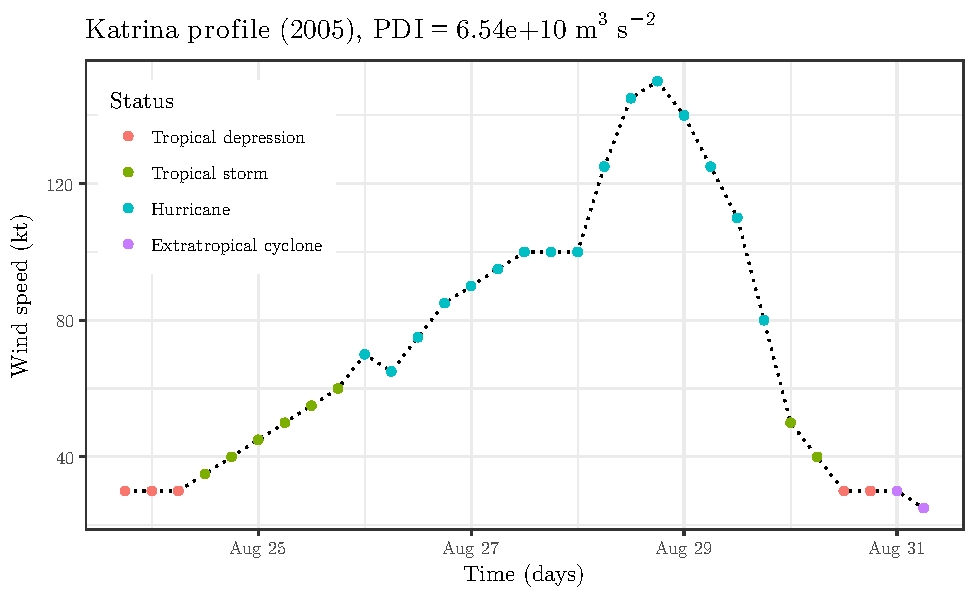
\includegraphics[width=\textwidth]{images/track-storm-katrina}
	\caption{Katrina (\texttt{AL122005}) sustained surface wind speed profile}
	\label{fig:katrina}
\end{figure}

The results found here are exactly the same found by \citeauthor{Corral2010}. In fact, Katrina is a good example of why removing additional records (as stated in~\cref{ssec:hurdat-import}) is essential to replicate their methodology and results. If we did the calculations by dynamically calculating the $\Delta t$ to take into account all the revised recorded data for each storm, which was our initial implementation, we would get $PDI = \SI{6.62 e10}{\cubic\m\per\square\s}$ instead of $PDI = \SI{6.54 e10}{\cubic\m\per\square\s}$. And this is not even the most extreme case; Katrina only has 3 additional records, whereas some storms have considerably more.

\sk
Since some storms are \texttt{UNNAMED}, we have also created the \inline{track_storm_by_id()} and \inline{get_pdi_by_id()} functions that do basically the same that standard functions defined above, but only require the storm ID. These two functions can be found in the script~\ref{scr:hurdat2_pdi_base}, in~\cref{app:code}).

One may wonder why we do not just stick to these \inline{*_by_id()} functions. The reason to define two separate functions is that in any realistic scenario, tracking storms or getting their $PDI$ by their name and year of occurrence is way faster and more intuitive for a researcher not familiarised with the Automated Tropical Cyclone Forecast (ATCF) cyclone number assignment system; in such cases \inline{*_by_id()} would only act as a fallback.

%-----------------------------------------------------------------
\subsubsection{Probability density}\label{ssec:dpdi}

Since the $PDI$ is a variable quantity, it is convenient to work with its probability density, $D(PDI)$. Let us recall that a probability density (in this case of tropical-cyclones $PDI$s) is defined as the probability that the value of the PDI is in a narrow interval,
\begin{align*}
	\left[ PDI, \, PDI + \dd{PDI} \right)
\end{align*}
normalized to the total number of occurrences, $N$, and divided by the length of the interval, $\dd{PDI}$, so that $\int_{0}^{\infty} D(PDI) \dd{PDI} \equiv 1$. That being so, the $D(PDI)$ is mathematically given by
\begin{align}\label{eq:dpdi}
	D(PDI) \equiv \frac{P[PDI \leq \text{value} < PDI + \dd{PDI}]}{\dd{PDI}} \approx \frac{n(PDI)}{N \dd{PDI}}
\end{align}

In \cite{Hergarten2002} \citeauthor{Hergarten2002} states that for variables distributed across a wide range of scales it is convenient to use a logarithmic binning instead of a linear binning, meaning that the bin widths increase accordingly to the scale of the variable. The main advantage of doing this is that the problem of low numbers of objects per bin at large sizes is less severe. Statistically, using a logarithmic binning means that for the $k$-th interval,
\begin{align}\label{eq:dpdi-log-bin}
	\dd{PDI} = c^{k-1}(c-1)m
\end{align}
where $c$ is a factor related to the size of each bin, and $m$ is an absolute minimum $PDI$ value. In this way, the value of $D(PDI)$ is associated to the whole interval
\begin{align}
	PDI_{min} = c^{k-1}m \leq PDI < PDI_{max} = c^{k} m
\end{align}

\citeauthor{Corral2010} have taken $c = \sqrt[5]{10} = 1.58$, which corresponds to 5 intervals per decade, and $m = \SI{e8}{\cubic\m\per\square\s}$. We have, however, taken the actual absolute minimum value for each basin, which is $m = \SI{1.84 e8}{\cubic\m\per\square\s}$ for both of them. It's important to note here that we have removed two clear outlying storms after doing a quick analysis of the $PDI$ data frames of both basins:
\begin{table}[H]
	\centering
	\begin{tabular}{l c c}
		\toprule
		\toprule
		Basin             & Storm ID          & $PDI$ (\si{\cubic\m\per\square\s}) \\
		\midrule
		North Atlantic    & \texttt{AL171988} & \num{1.25 e8} \\
		Northeast Pacific & \texttt{EP231989} & \num{2.35 e7} \\
		\bottomrule
	\end{tabular}
	\caption{Outlying storms judging by their $PDI$ value}
	\label{tab:pdi-outliers}
\end{table}

Since we want to plot the $D(PDI)$, it's useful to choose a single point of the interval, $PDI\sast$, to be representative of the probability density. The exact calculation of $PDI\sast$ is fairly complex, as it would require to know the mathematical form of the probability distribution beforehand. We know, however, that geophysical systems are generally described by a Pareto power law distribution~\cite{Hergarten2002}. Therefore, a reasonable estimation of $PDI\sast$ is the geometric mean of the limits of the interval:
\begin{align}\label{eq:pdi-star}
	PDI\sast = \sqrt{PDI_{min} PDI_{max}}
\end{align}

\begin{subequations}
The error bars for each interval are estimated from the standard deviation of the probability density:
\begin{align}\label{eq:pdi-error}
	\epsilon(PDI) &\equiv \epsilon_{rel} (PDI) D(PDI)
\end{align}
where the relative error follows a binomial distribution:
\begin{align}
	\epsilon_{rel} (PDI) &= \sqrt{\frac{1-P}{n}} \approx \frac{1}{\sqrt{n}}
\end{align}
\end{subequations}

\sk
The calculation of the $PDI$ probability density looks quite complex, but it's really not that complicated to do using R. The process consists in creating an empty data frame containing the values of $PDI_{min}$ and $PDI_{max}$ for each individual bin following \eqref{eq:dpdi-log-bin}, being \inline{pdi.bin}~$\equiv \dd{PDI}$ the size of each bin. The computation of $PDI\sast$, \inline{ndpdi}~$= n$, and \inline{length(hurr.obs.pdi}\texttt{\textbf{\$}}\inline{storm.pdi)}~$= N$ is straightforward. Once we have calculated those, the values of \inline{dpdi}~$= D(PDI)$ and \inline{pdi.error}~$=\epsilon(PDI)$ are calculated using \eqref{eq:dpdi} and \eqref{eq:pdi-error}, respectively:
\begin{lstlisting}[caption=Function to calculate the $D(PDI)$ in a range of years, label=snp:hurdat-dpdi]
get_dpdi <- function(hurr.obs.pdi, years){
	hurr.obs.pdi <- hurr.obs.pdi %>%
		filter(storm.year %in% years)
	c <- 10^(1/5)
	m <- min(hurr.obs.pdi$storm.pdi)
	dpdi.df <- data.frame()
	for (i in 1:20) {
		dpdi.df <- rbind(dpdi.df, c(c^(i-1)*m, c^(i)*m))
	}
	colnames(dpdi.df) <- c("pdi.min", "pdi.max")
	dpdi.df <- dpdi.df %>%
		mutate(pdi.star = sqrt(pdi.min * pdi.max),
					 pdi.bin = pdi.max - pdi.min) %>%
		rowwise() %>%
		mutate(ndpdi = sum(hurr.obs.pdi$storm.pdi >= pdi.min &
											 hurr.obs.pdi$storm.pdi <= pdi.max),
					 dpdi = ndpdi/(length(hurr.obs.pdi$storm.pdi)*pdi.bin),
					 pdi.error = dpdi / sqrt(ndpdi) ) %>%
		filter(dpdi != 0)
	return(dpdi.df)
}
\end{lstlisting}
Note that since we do not know the absolute maximum $PDI$ value in advance, we create a few more bins than necessary, giving us the following range:
\begin{align*}
	PDI \in [ m, \, c^{20} m ) = [ \num{1.84 e8}, \, \num{1.84 e12})\, \si{\cubic\m\per\square\s}
\end{align*}
After doing the calculations previously described, we just need to delete the rows (bins) with no value for $n$ (or $D(PDI)$ to be more precise). It's important to notice that this short routine won't affect the compile times in any significant way.

The \inline{plot_dpdi()} function that allows us to plot the $D(PDI)$ against the $PDI$ using this logarithmic binning is defined in the script~\ref{scr:hurdat2_pdi_base}, in~\cref{app:code}). In figures~\ref{fig:dpdi-natl} and~\ref{fig:dpdi-epac} we can see probability density analysis for the N.~Atl. and E.~Pac. basins for the 1966-2016 period.
\begin{figure}[H]
	\centering
	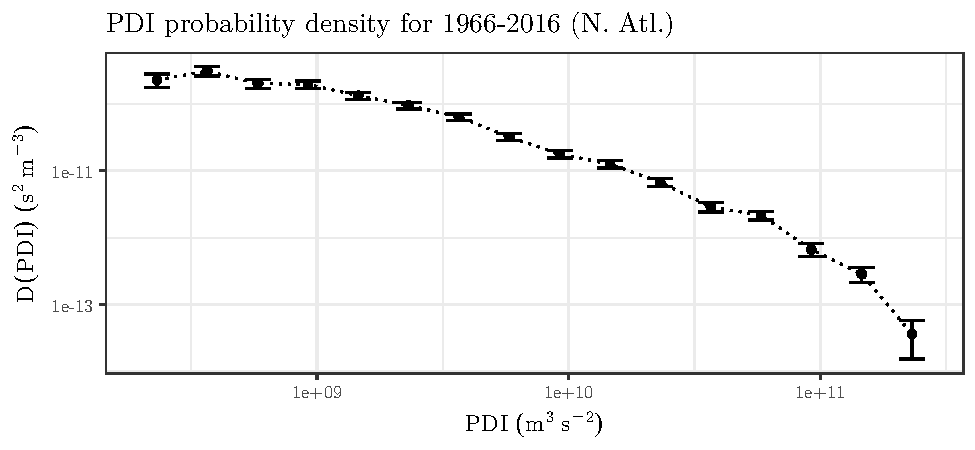
\includegraphics[width=\textwidth]{images/dpdi-natl}
	\caption{$D(PDI)$ distribution for the North Atlantic Ocean}
	\label{fig:dpdi-natl}
\end{figure}

\begin{figure}[H]
	\centering
	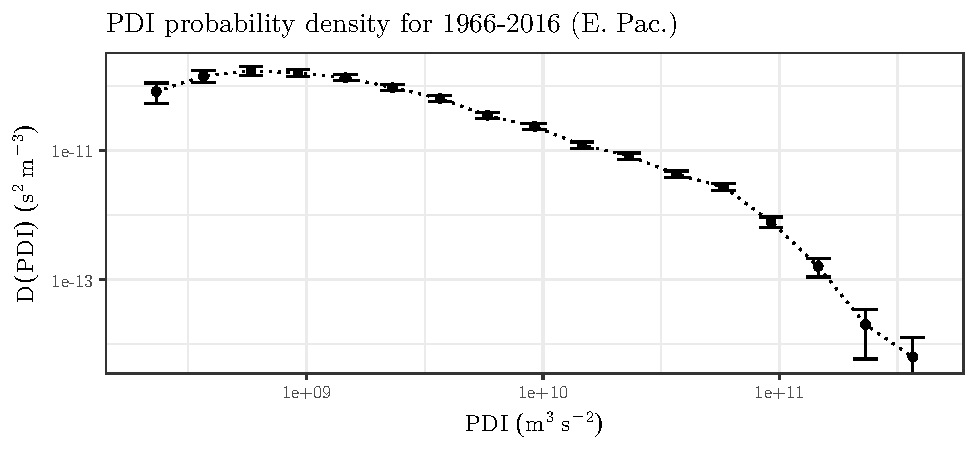
\includegraphics[width=\textwidth]{images/dpdi-epac}
	\caption{$D(PDI)$ distribution for the Northeast Pacific Ocean}
	\label{fig:dpdi-epac}
\end{figure}

As we can see, both distributions are essentially the same, being the end of the tail the only remarkable difference. It is apparent how the tail has a longer range when the size of the region is increased (the North Atlantic Ocean is about three times bigger than the Northeast Pacific Ocean). In \cite{Corral2010} \citeauthor{Corral2010} go into a fair amount of detail on the effect of the finite size of basins, both from a physical and a statistical point of view, showing that the finite size delimits the evolution and lifetime of hurricanes.

\sk
What we want to focus on, however, is the causal relationship between increasing hurricane intensity and increasing sea surface temperature (SST) proposed by \citeauthor{Trenberth2005} in~\cite{Trenberth2005}. In the text \citeauthor{Trenberth2005} states that higher SSTs are associated with increased water vapour in the lower troposphere; both higher SSTs and increased water vapour tend to increase the energy available for atmospheric convection and the energy available to tropical-cyclones as a consequence.

The hypothesis is, therefore, that separating the $PDI$ data by low-SST and high-SST years, we should get two similar $D(PDI)$ distributions with one major difference: high-SST years should have a longer tail on account of having more available energy from the sea. For this separation (or classification) process we will follow the methodology used by \citeauthor{Corral2010} in~\cite{Corral2010}, which is a variation of the methodology proposed by \citeauthor{Webster2005} in~\cite{Webster2005}.
